% ============================================================================
\chapter{제안 방법}\label{ch:method}
% ============================================================================

\section{전체 구성}\label{sec:method_overview}

\figref{fig:pipeline}은 본 연구의 전체 흐름이다. 1단계에서 두 공개 데이터셋을 통일된 형식으로 변환하고
분할을 설계하며(\chapref{ch:dataset}), 2단계에서 기준 모델의 용량을 정한다(\secref{sec:exp_baseline}).
3단계에서 경계 정교화 모듈과 경계 인식 손실을 적용하고(\secref{sec:brm}--\secref{sec:dualpath}),
4단계에서 사후 양자화로 배포 형식을 만든다(\secref{sec:quant}). 마지막으로 배포 환경에 따라
CPU에서는 OpenVINO INT8, GPU에서는 ONNX FP16을 선택한다.

\begin{figure}[htbp]
  \centering
  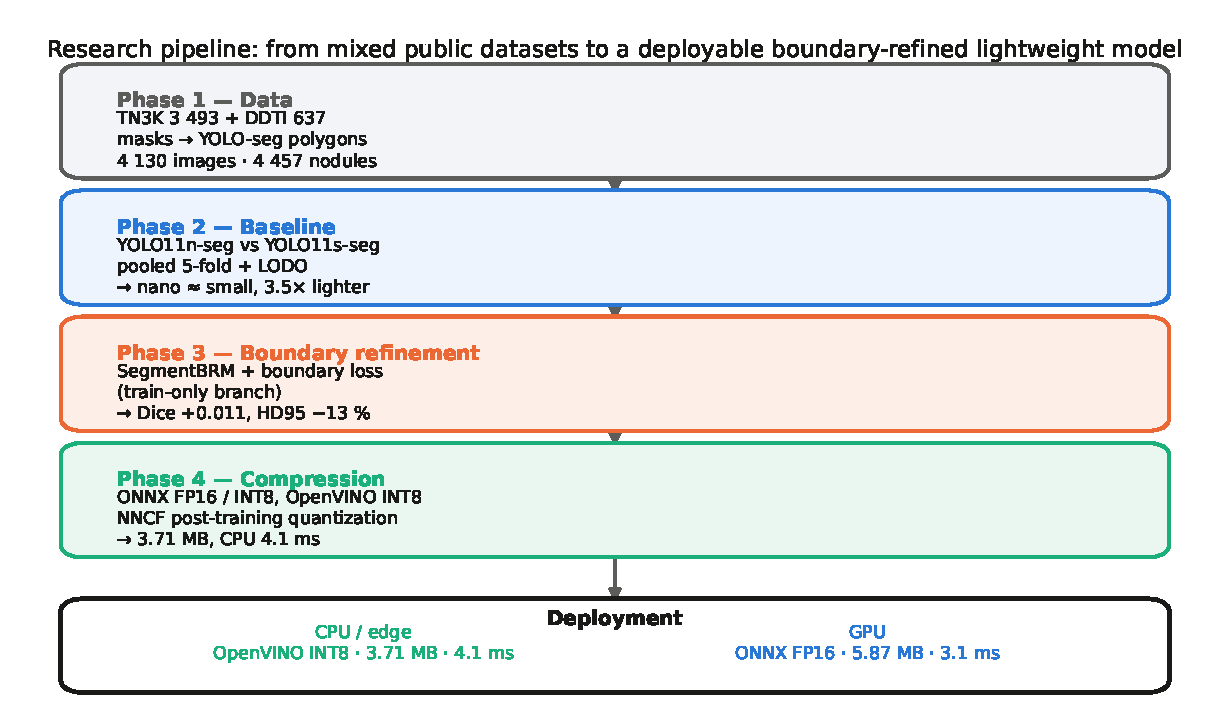
\includegraphics[width=0.92\linewidth]{fig8_pipeline}
  \caption[연구 파이프라인.]{연구 파이프라인. 데이터 정비부터 배포 형식 선택까지의 네 단계와 각 단계의 핵심 결과.}
  \label{fig:pipeline}
\end{figure}

\section{기반 모델: YOLOv11-seg}\label{sec:base_model}

기반 모델은 YOLOv11n-seg\citep{jocher2024yolo11}이다. 640$\times$640 입력에 대해 백본(0--10층,
1,365,472개 파라미터)이 C3k2·SPPF·C2PSA 블록으로 특징을 추출하고, 넥(11--22층, 793,696개)이
FPN·PAN 구조로 스트라이드 8, 16, 32의 세 특징 맵 $\{F_3, F_4, F_5\}$를 만든다. 세 특징 맵의 격자 수를
합한 8,400개 위치가 각각 하나의 예측 후보가 된다.

분할 헤드는 YOLACT\citep{bolya2019yolact}의 프로토타입 방식을 따르며 세 경로로 이루어진다.

\begin{itemize}
  \item \textbf{검출 경로}: 각 위치에서 상자를 DFL\citep{li2020gfl} 분포로 회귀하고 클래스 점수를 예측한다.
  \item \textbf{계수 경로}(\texttt{cv4}): 각 위치에서 길이 $K=32$의 마스크 계수 벡터 $\bm{c}\in\mathbb{R}^{K}$를 예측한다.
    스케일마다 3$\times$3 합성곱 두 개와 1$\times$1 합성곱 하나로 구성된다.
  \item \textbf{프로토타입 경로}(Proto): 가장 고해상도인 $F_3$(80$\times$80)를 입력받아
    3$\times$3 합성곱, 2배 전치 합성곱, 3$\times$3 합성곱, 1$\times$1 합성곱을 거쳐
    입력의 1/4 해상도(160$\times$160)에서 $K$개의 프로토타입 $\bm{P}\in\mathbb{R}^{K\times 160\times 160}$를 만든다.
\end{itemize}

객체 $i$의 마스크는 계수와 프로토타입의 선형 결합으로 만들어진다.
\begin{equation}
  \hat{\bm{m}}_i = \sigma\!\left(\sum_{k=1}^{K} c_{ik}\,\bm{P}_k\right) \in [0,1]^{160\times160}
  \label{eq:proto}
\end{equation}
여기서 $\sigma$는 시그모이드 함수이다. 추론 시에는 이 마스크를 예측 상자 안으로 잘라 원본 해상도로 키운다.
프로토타입 $\bm{P}$는 한 영상의 모든 객체가 공유하므로, \eqnref{eq:proto}의 마스크 품질은 결국
프로토타입이 경계를 얼마나 잘 표현하느냐에 달려 있다. 제안 방법은 이 공유 프로토타입을 개선 대상으로 삼는다.

\section{경계 정교화 모듈: \BRM}\label{sec:brm}

\figref{fig:architecture}는 제안 모델의 구조이다. \BRM{}은 기존 분할 헤드를 대체하지 않고 확장한다.
검출·계수·프로토타입의 세 경로는 그대로 두고, 프로토타입 출력 $\bm{P}$에서 보조 경계 분기 $g_\phi$ 하나를
추가로 갈라낸다.
\begin{equation}
  \hat{\bm{e}} = g_\phi(\bm{P}) = \mathrm{Conv}_{1\times1}^{16\rightarrow1}\Big(\mathrm{SiLU}\big(\mathrm{BN}(\mathrm{Conv}_{3\times3}^{32\rightarrow16}(\bm{P}))\big)\Big)
  \in \mathbb{R}^{1\times160\times160}
  \label{eq:edge_branch}
\end{equation}
$\hat{\bm{e}}$는 각 픽셀이 결절 경계에 속할 로짓이다. 분기의 파라미터는 3$\times$3 합성곱 4,608개, 배치 정규화
32개, 1$\times$1 합성곱 17개로 모두 4,657개이며, 전체 모델(2,847,460개)의 0.16\%이다.

이 분기를 프로토타입 뒤에 둔 이유는 다음과 같다. 경계 분기가 계산하는 손실의 기울기는 $g_\phi$를 거쳐
$\bm{P}$로, 다시 프로토타입 경로와 넥, 백본으로 전파된다. 즉 경계 감독 신호가 모든 객체 마스크가 공유하는
프로토타입에 직접 작용하여, 프로토타입이 경계 정보를 담도록 유도한다. 분기는 이 유도 역할만 하고
마스크 생성에는 관여하지 않으므로, 학습이 끝나면 제거해도 \eqnref{eq:proto}의 결과는 달라지지 않는다.

\begin{figure}[htbp]
  \centering
  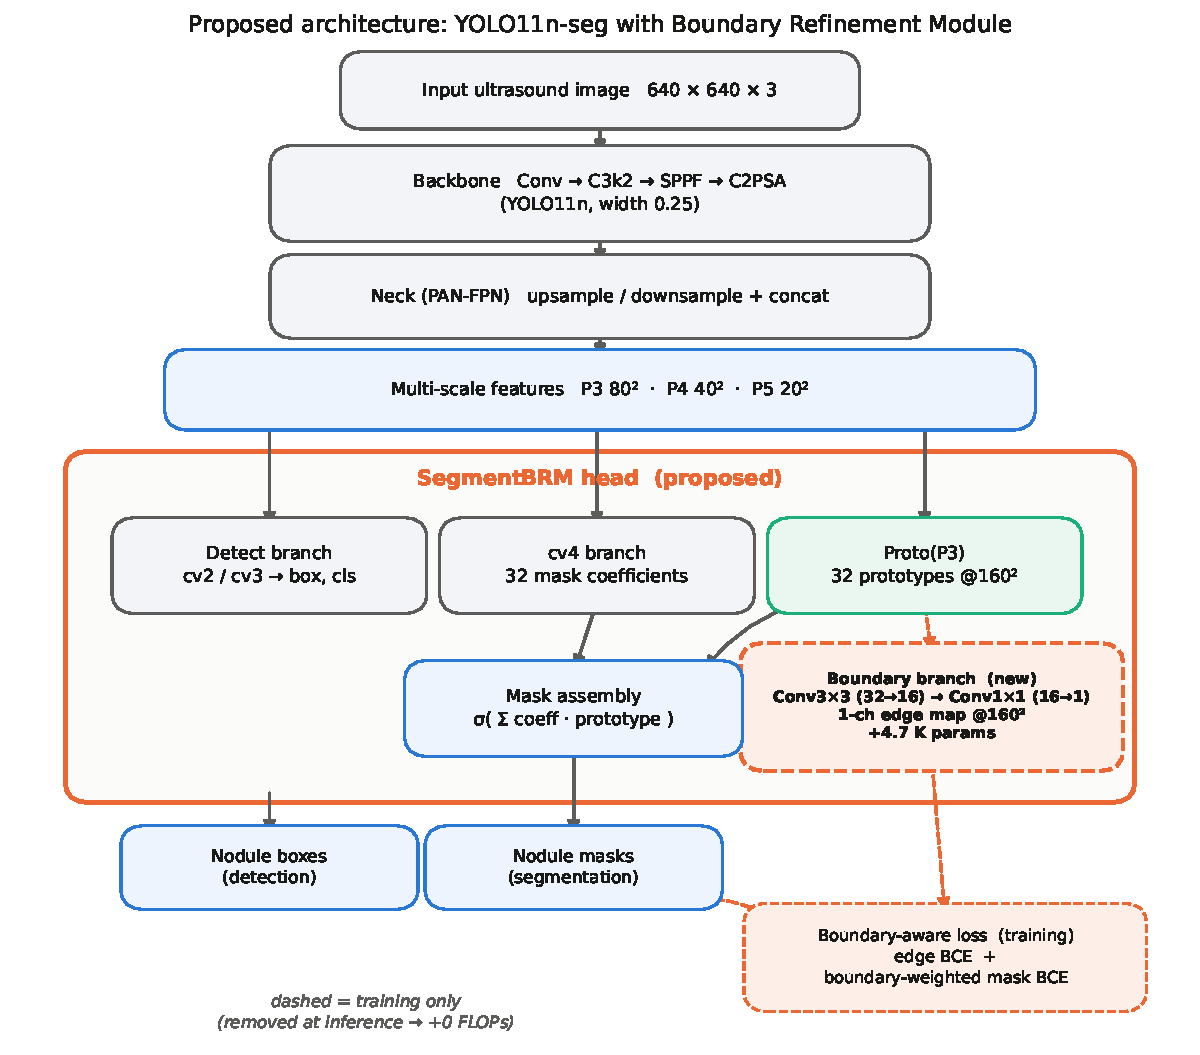
\includegraphics[width=0.85\linewidth]{fig5_architecture}
  \caption[제안 모델의 구조.]{제안 모델의 구조. 점선으로 표시한 경계 분기와 경계 인식 손실은 학습 때만 사용되며,
    추론 그래프에는 포함되지 않는다.}
  \label{fig:architecture}
\end{figure}

\section{경계 인식 손실}\label{sec:boundary_loss}

\subsection{형태학적 경계 밴드}

이진 마스크 $\bm{M}$의 경계 밴드를 형태학적 기울기로 정의한다.
\begin{equation}
  \mathcal{B}(\bm{M}) = \mathrm{clip}\big(\dil_{3\times3}(\bm{M}) - \ero_{3\times3}(\bm{M}),\ 0,\ 1\big)
  \label{eq:band}
\end{equation}
팽창과 침식은 각각 3$\times$3 최대 풀링과 부호를 바꾼 최대 풀링으로 구현하므로, 학습 파라미터가 없고
GPU에서 추가 비용이 거의 없다. 마스크 해상도(160$\times$160)에서 밴드의 폭은 경계 안팎으로 한 픽셀씩
두 픽셀이며, 이는 640 입력 기준 약 8픽셀에 해당한다. \figref{fig:boundary_loss}는 실제 정답 마스크에서
계산한 밴드와 가중치 맵이다.

\begin{figure}[htbp]
  \centering
  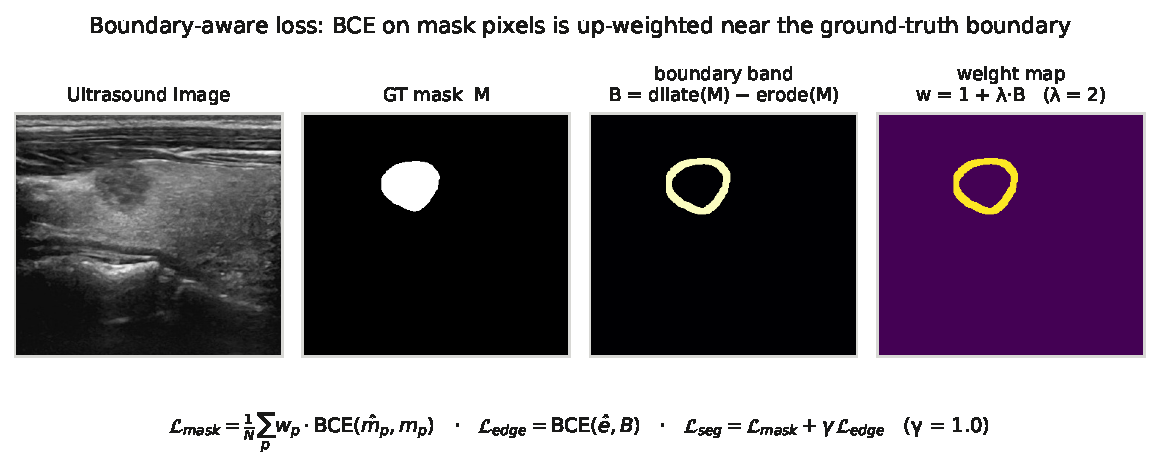
\includegraphics[width=\linewidth]{fig7_boundary_loss}
  \caption[경계 인식 손실의 구성.]{경계 인식 손실의 구성. 초음파 영상, 정답 마스크 $\bm{M}$, 형태학적 경계 밴드 $\mathcal{B}(\bm{M})$,
    가중치 맵 $\bm{w} = 1 + \lambda\mathcal{B}$ ($\lambda=2$).}
  \label{fig:boundary_loss}
\end{figure}

\subsection{경계 가중 마스크 손실}

YOLOv11-seg의 마스크 손실은 양성으로 할당된 각 예측 $j$에 대해, 대응하는 정답 상자 영역 $R_j$ 안의 픽셀별
이진 교차 엔트로피를 평균한다. 제안 손실은 여기에 경계 가중치를 곱한다.
\begin{gather}
  w_p = 1 + \lambda\,\mathcal{B}(\bm{m}_j)_p \label{eq:weight}\\
  \mathcal{L}_{\text{mask}}^{\text{BW}} = \frac{1}{N_{\text{fg}}}\sum_{j=1}^{N_{\text{fg}}} \frac{1}{|R_j|}
    \sum_{p\in R_j} w_p\,\BCE\!\big(\bm{c}_j^{\top}\bm{P}_{:,p},\ m_{jp}\big)
  \label{eq:mask_bw}
\end{gather}
$\bm{m}_j$는 예측 $j$에 할당된 정답 결절의 마스크, $N_{\text{fg}}$는 양성 예측 수이다.
$\lambda=0$이면 원래의 마스크 손실과 같다. $\lambda>0$이면 경계 밴드 픽셀의 오차가 내부 픽셀보다
$(1+\lambda)$배 크게 반영되어, 학습 신호가 경계에 집중된다.

\subsection{보조 경계 손실}

경계 분기의 출력 $\hat{\bm{e}}$는 영상 전체 결절의 합집합 마스크 $\bm{S}$의 경계 밴드를 정답으로 학습한다.
\begin{equation}
  \mathcal{L}_{\text{edge}} = \frac{1}{N_b H W}\sum_{b=1}^{N_b}\sum_{p} \BCE\!\big(\hat{e}_{bp},\ \mathcal{B}(\bm{S}_b)_p\big)
  \label{eq:edge_loss}
\end{equation}
$N_b$는 배치 크기, $H\times W = 160\times160$이다. 정답 마스크는 데이터 로더가 제공하는 인스턴스 마스크를
마스크 해상도로 최근접 보간한 뒤 0보다 큰 픽셀을 전경으로 하여 만든다.

\subsection{전체 손실}

전체 손실은 YOLOv11-seg의 손실 구성에 두 경계 항을 더한 것이다.
\begin{equation}
  \mathcal{L} = N_b\Big[\,\lambda_{\text{box}}\mathcal{L}_{\text{box}} + \lambda_{\text{cls}}\mathcal{L}_{\text{cls}}
  + \lambda_{\text{dfl}}\mathcal{L}_{\text{dfl}}
  + \lambda_{\text{box}}\big(\mathcal{L}_{\text{mask}}^{\text{BW}} + g\,\mathcal{L}_{\text{edge}}\big)\Big]
  \label{eq:total_loss}
\end{equation}
$\mathcal{L}_{\text{box}}$는 CIoU 손실, $\mathcal{L}_{\text{cls}}$는 분류 BCE, $\mathcal{L}_{\text{dfl}}$는
분포 초점 손실이며, 가중치는 YOLOv11 기본값 $\lambda_{\text{box}}=7.5$, $\lambda_{\text{cls}}=0.5$,
$\lambda_{\text{dfl}}=1.5$를 그대로 사용하였다. Ultralytics 구현은 마스크 손실에 상자 손실과 같은 가중치
$\lambda_{\text{box}}$를 쓰므로, 경계 항도 같은 가중치를 공유하도록 하여 원래 손실들과 크기 균형을 맞췄다.
경계 항의 두 계수, 즉 보조 손실 가중치 $g$와 경계 강조 계수 $\lambda$는 \secref{sec:sweep}의 스윕으로
$g=1.0$, $\lambda=2.0$으로 정하였다. 두 경계 항은 학습 로그에서 분할 손실 항목에 합산되므로,
4개 항목으로 이루어진 기존 손실 기록 형식은 바뀌지 않는다. \algref{alg:train_step}은 학습 한 단계의 절차이다.

\begin{algorithm}[htbp]
\caption{\BRM{} 학습 한 단계}\label{alg:train_step}
\begin{algorithmic}[1]
\Require 배치 영상 $\bm{X}$, 정답 상자·클래스, 인스턴스 마스크; 계수 $g$, $\lambda$
\State $\{F_3,F_4,F_5\} \gets \mathrm{Neck}(\mathrm{Backbone}(\bm{X}))$
\State 상자·클래스 예측, 마스크 계수 $\bm{c}$ $\gets$ 검출 경로, 계수 경로$(F_3,F_4,F_5)$
\State $\bm{P} \gets \mathrm{Proto}(F_3)$; \quad $\hat{\bm{e}} \gets g_\phi(\bm{P})$ \Comment{학습 모드에서만 계산}
\State 과제 정렬 할당기로 양성 예측과 정답 결절을 짝짓는다
\State $\mathcal{L}_{\text{box}}, \mathcal{L}_{\text{cls}}, \mathcal{L}_{\text{dfl}}$ 계산
\For{각 양성 예측 $j$}
  \State $\bm{w} \gets 1 + \lambda\,\mathcal{B}(\bm{m}_j)$ \Comment{\eqnref{eq:band}, \eqnref{eq:weight}}
  \State 상자 $R_j$ 안에서 $\bm{w}\odot\BCE(\bm{c}_j^{\top}\bm{P},\ \bm{m}_j)$의 평균을 누적
\EndFor
\State $\mathcal{L}_{\text{edge}} \gets \BCE(\hat{\bm{e}},\ \mathcal{B}(\bm{S}))$ \Comment{\eqnref{eq:edge_loss}}
\State \eqnref{eq:total_loss}로 $\mathcal{L}$을 구하고 역전파하여 모든 파라미터를 갱신
\end{algorithmic}
\end{algorithm}

\section{학습--추론 분리와 추론 비용}\label{sec:dualpath}

\figref{fig:dual_path}는 같은 모델이 학습과 추론에서 서로 다른 경로로 동작하는 모습이다.
학습 모드에서 \BRM{}은 (검출 출력, 마스크 계수, 프로토타입, 경계 로짓)의 네 값을 반환하고, 손실 함수는
네 번째 값이 있을 때만 경계 항을 계산한다. 추론 모드와 ONNX·OpenVINO 변환 모드에서는 경계 분기
$g_\phi$를 아예 호출하지 않고, 기존 분할 헤드와 똑같은 형태의 출력만 반환한다.

따라서 배포되는 연산 그래프는 베이스라인과 동일하다. 실제로 640$\times$640 입력에서 측정한 추론 연산량은
베이스라인과 제안 모델 모두 9.73 GFLOPs로 같았다(\tabref{tab:brm_main}). 경계 분기의 가중치 4,657개는
PyTorch 체크포인트 파일에만 남아 파일 크기를 6.00 MB에서 6.01 MB로 늘릴 뿐, 변환된 추론 그래프에는
포함되지 않는다. 이 분리 덕분에 경계 품질 향상이 추론 비용 증가라는 대가를 요구하지 않는다.

\begin{figure}[htbp]
  \centering
  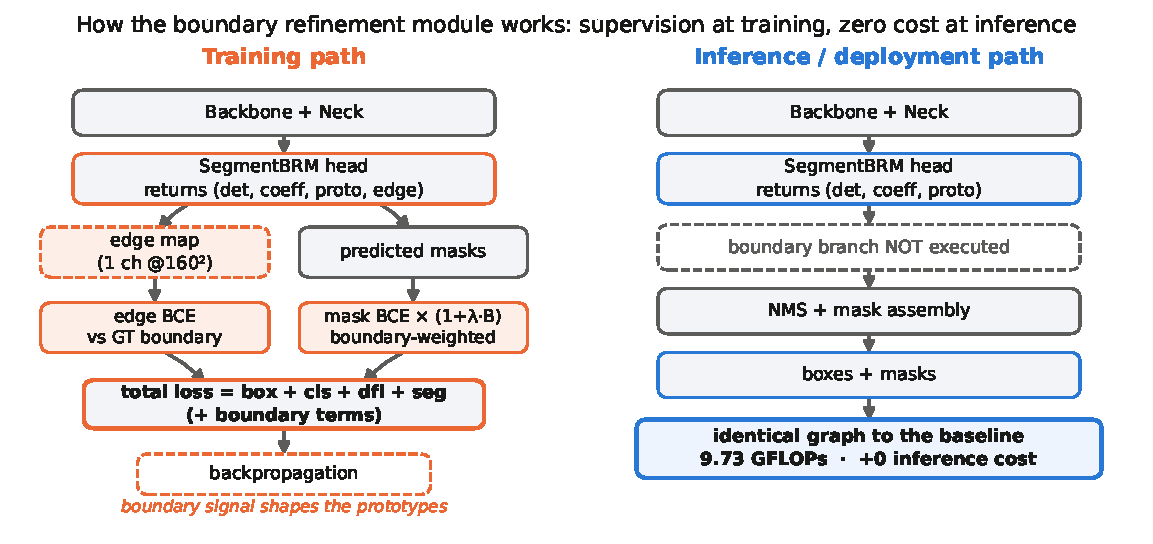
\includegraphics[width=\linewidth]{fig6_dual_path}
  \caption[학습 경로와 추론 경로.]{학습 경로와 추론 경로. 학습 때는 경계 분기가 프로토타입에 경계 신호를 전달하고,
    추론 때는 분기가 실행되지 않아 베이스라인과 같은 그래프가 된다.}
  \label{fig:dual_path}
\end{figure}

\section{사후 양자화 파이프라인}\label{sec:quant}

제안 모델을 재학습 없이 배포 형식으로 바꾸기 위해 다섯 가지 정밀도를 준비하였다.

\paragraph{ONNX FP32 / FP16.} Ultralytics 변환 기능으로 opset 13의 ONNX 그래프를 만들고 그래프 단순화를
적용하였다. FP16은 GPU에서 반정밀도로 변환하였다.

\paragraph{ONNX Runtime 정적 INT8.} ONNX FP32 모델에 전처리(형상 추론·그래프 정리)를 적용한 뒤, ONNX Runtime의
정적 양자화를 QDQ 형식으로 수행하였다. 가중치는 채널별 부호 있는 INT8, 활성값은 부호 없는 INT8이며,
캘리브레이션에는 TN3K 학습·검증 분할에서 무작위로 뽑은 150장(시드 42)을 추론과 같은 방식
(640 레터박스, 0--1 정규화)으로 전처리하여 사용하였다. 채널별 QDQ 양자화는 opset 13 이상에서만 유효한
그래프가 만들어진다.

이 과정에서 중요한 실패를 확인하였다. 그래프 전체를 양자화하면 모든 클래스 점수가 0이 되어 아무것도
검출되지 않는다. 헤드의 시그모이드 직전 로짓과 DFL 분포처럼 출력 단의 작은 값 차이가 결과를 좌우하는
연산이 8비트 해상도로 표현되면서 정보가 손실된 것으로 추정된다. OpenVINO 변환 경로가 바로 이 연산들을
양자화에서 제외하도록 설계되어 있다는 점(아래)도 이 해석을 뒷받침한다. 그래서 분할 헤드(그래프의
\texttt{/model.23/} 이하 119개 노드)를 양자화 대상에서 제외하고 부동소수점으로 남겼으며, 이렇게 하자
검출 출력이 정상으로 돌아왔다.

\paragraph{OpenVINO INT8.} Ultralytics의 OpenVINO 변환 기능으로 FP32 IR을 만든 뒤 NNCF\citep{kozlov2020nncf}로
사후 양자화하였다. 양자화 방식은 NNCF의 MIXED 프리셋(가중치 대칭, 활성값 비대칭)이며, 캘리브레이션에는
해당 fold의 검증 분할 영상을 사용하였다. 이 경로에서는 헤드 전체가 아니라 헤드 안의 덧셈·뺄셈·곱셈·나눗셈
연산, DFL 연산, 그리고 모든 시그모이드 연산만 양자화 범위에서 제외된다. 즉 헤드의 합성곱, 특히 160$\times$160
해상도에서 동작하는 프로토타입 경로의 합성곱은 INT8로 바뀐다. 두 INT8 경로의 지연 시간 차이는 대부분
이 제외 범위의 차이에서 비롯된다(\secref{sec:disc_quant}).

\paragraph{배포 형식 선택.} 정확도는 모든 정밀도에서 같은 held-out 집합과 같은 평가 코드로 다시 측정하였다.
INT8 모델은 배포 대상인 CPU에서, FP32·FP16 모델은 GPU에서 평가하였다.
